\section{Organisation}

\subsection{Déroulement}

Ce projet se déroule du jeudi 4 mai au jeudi 25 juin (inclu). Vous trouverez sur les sites des deux 
classes les calendriers actualisés des séances de TP. 

%Lorsqu'un nom de groupe est indiqué lors d'une séance, ce groupe doit assister à la séance. 
% Mais à tout moment, il est possible à chacun d'assister à une autre séance de TP, quel 
% que soit son groupe ou sa classe (dans la limite des places disponibles).\\

Nous vous demandons d'assister à trois séances, au minimum. 
Vous êtes libres de choisir la date des séances de TP dans la limite des places disponibles (les étudiants devant avoir TP ce jours là étant prioritaires). 
Avec l'accord de votre enseignant, vous pouvez aussi changer de groupe/enseignant (le mieux est de faire un échange). 

Vous devrez rendre votre projet au plus tard le vendredi 26 juin à 22 heures. Ces projets seront évalués. Le voyage de classe et les conseils de 
classe n'ayant lieu que quelques jours après cette date, n'hésitez pas à rendre votre projet plus tôt si vous avez 
fini en avance, cela facilitera le travail de correction de vos enseignants.


\textbf{Attention}:
\begin{itemize}
\item Les projets incomplets ou en retard seront notés $0$ et/ou signalés sur le bulletins.
\item En  pratique, un  projet informatique est  source d'innombrables
  problèmes.   Ces  problèmes  doivent  être  anticipés,  ce  qui  est
  difficile car ils sont imprévisibles.  Il faut donc essayer de finir
  en avance sur  la date prévue pour avoir une  marge de sécurité.  Si
  aucun  problème ne  se  pose,  vous aurez  alors  la possibilité  de
  peaufiner votre  projet.  \textbf{En  aucun cas, ces  problèmes ne  sont une
  excuse  valable  pour  rendre  en retard}.   Par  exemple,  si  votre
  ordinateur  plante la  veille  du jour  du rendu  et  que vous  vous
  apercevez  alors  que la  clé  USB  sur  laquelle vous  faisiez  vos
  sauvegardes est  passée à  la machine  à laver,  cela n'est  pas une
  excuse valable.
\end{itemize}

\subsection{Équipes}
Le projet  se fait par binômes,  les binômes devant être avec le même
enseignant (sauf exception validée par vos enseignants).  Si  le nombre  de membres  de votre  groupe de  TP est
impair (et seulement dans ce  cas), votre enseignant peut autoriser un
unique monôme  ou un  unique trinôme (consultez-le  immédiatement pour
savoir si c'est votre cas).

\subsection{Suggestion de progression}

\subsubsection{Première séance de TP} Choisir un sujet, récupérer des données en lignes et s'entraîner à
manipuler des bases de données SQL avec \texttt{sqlite3} et \texttt{Python}
en utilisant la base de données de films présentée en cours.

\subsubsection{Deuxième séance} 
Lors de  la deuxième  séance de  TP, vous  devez déjà  avoir largement
commencé  votre projet.   Vous devez  avoir  sur vous (en début de séance) un cahier  des
charges dactylographié indiquant :
\begin{enumerate}
\item vos noms ;
\item le sujet que vous avez choisi.
\item ce que vous comptez faire sur le sujet (à quoi votre programme  ressemblera pour l'utilisateur final, quelles seront les questions à poser, le schéma de la base de données).
\end{enumerate}
Vous pourrez alors poser des questions à votre enseignant. Si celui-ci
valide  votre  cahier  des  charges,   vous le lui  rendrez.  Il  pourra
également, s'il  l'estime préférable,  vous demander d'y  apporter des
modifications et vous dira dans ce cas combien de temps il vous laisse
pour faire ces modifications et lui rendre la nouvelle version.

\subsubsection{Troisième séance}
C'est le moment de résoudre les derniers petits problèmes avec l'aide
de votre enseignant et de voir si le rapport que vous avez rédigé
convient ou ce qu'il faut adapter à ce rapport.

\subsubsection{Après la troisième séance}
Au moment de rendre votre TP, vous devez rendre à votre enseignant:
\begin{enumerate}
\item Un compte-rendu dactylographié, au format PDF.
\item Votre programme \python.
\item Votre base de données.
\end{enumerate}
Vous devrez impérativement respecter les instructions de nommage suivantes : 
\begin{itemize}
    \item le nom de votre fichier PDF sera \texttt{dupont-durand-projet.pdf},
    \item le nom de votre fichier python sera \texttt{dupont-durand-projet.py},
    \item le nom de votre base de données sera \texttt{dupont-durand-projet.sqlite},
\end{itemize}
où \texttt{dupont} et
\texttt{durand} sont à  remplacer par vos noms (en minuscules, sans espaces, sans
caractères accentués ni caractères spéciaux).

\subsubsection{Compte-rendu}

Le compte-rendu devra au minimum comporter les points suivants : 
\begin{itemize}
    \item noms et prénoms des membres du groupe ; 
    \item thème du projet ; 
    \item origine de la base de données et traitement apporté à la base de données si cette dernière a été prise en ligne ; 
    \item schéma entité-association de la base de données ; 
    \item instructions et explications de prise en main de votre programme (quelques exemples seraient appréciés, surtout s'il n'y a pas d'interface graphique) ; 
    \item exemple de requête complexe (actions à mener pour produire cette requête en utilisant votre programme et code SQL correspondant). 
\end{itemize}

\section{Sujet}

\subsection{Contraintes}
Vous pouvez choisir le sujet que vous voulez sous réserve du respect
absolu des contraintes suivantes (en cas de doute, demandez à votre
enseignant):

\begin{enumerate}
\item Votre programme doit être écrit en python version 3. \textbf{Pas
    python2}.
\item Pour lancer votre programme, il doit être suffisant d'ouvrir un
  terminal, de se placer dans le répertoire où se situe votre fichier
  \texttt{dupont-durand-projet.py} et de taper \texttt{python3
    dupont-durand-projet.py}.
\item Votre  programme doit manipuler  une base de  données comportant
  plusieurs tables et certaines des  requêtes que vous ferez sur cette
  base de  données doivent  être non triviales. On  considérera qu'une
  requête  qui manipule  des  données venant  d'au  moins deux  tables
  différentes est non triviale. Les tables de votre base doivent être
  raisonnablement remplies (on ne vous demande pas des milliers de
  données mais si vos tables ne contiennent que 5 lignes chacune, il
  y a sans doute un problème).
\item Votre programme doit être  un programme utilisable par quelqu'un
  qui ne connaît rien à python et doit lui apporter (un petit) quelque chose.
\end{enumerate}

\subsection{Exemples de sujets}

Voici quelques exemples de sujets. Vous pouvez prendre un sujet
totalement différent, vous pouvez également prendre un des sujets
suggérés ci-dessous et l'adapter à votre goût.

\subsubsection{Manipulation d'une base de données cinématographiques}
Grâce à \texttt{sqlite3}, vous pouvez créer un fichier de base de
données \texttt{cinema.sqlite} comportant les tables présentées en cours,
puis vous pourrez importer les données fournies dans les fichiers
\texttt{.csv} du TP précédent. Puis vous écrirez en Python un
programme qui permettra à un utilisateur de consulter voire de
modifier cette base de données.

\subsubsection{Gestion de recettes de cuisine}
Vous créerez une base comportant des recettes de cuisine. Pour chaque
recette, il pourra être intéressant de fournir la liste des
ingrédients possible (et des quantités). On pourrait vouloir chercher
des recettes comportant certains ingrédients ou au contraire ne
comportant pas certains ingrédients. On peut aussi imaginer d'associer
à chaque ingrédient un prix et utiliser les capacités de SQL pour
calculer le prix d'une recette en fonction des ingrédients et des
quantités, etc.

\subsubsection{Micro-Parcoursup}
Créer une base représentant une liste de candidats pour une formation.
Aux  différents candidats,  on veut  pouvoir associer  son lycée,  les
matières qu'il a suivi et les  moyennes qu'il a eues dans ces matières
en terminale (premier  et second trimestre), ainsi  que son classement
dans  cette matière  et  l'effectif de  son  groupe-classe pour  cette
matière.  On  veut ensuite  pouvoir trier des  candidats par  ordre de
moyenne,  mettre une  priorité (donc  un classement)  pour les  places
d'internat en fonction de sa moyenne  générale et de la distance de sa
ville d'origine (qu'on estimera être celle de son lycée) à la ville où
a lieu la formation demandée.  Pour calculer cette distance, on pourra
gérer    une    table    de     villes    avec    leurs    coordonnées
géographiques et
se contenter de calculer la distance à vol d'oiseau.

\subsubsection{Gestion de chambres d'hôtel}
On veut gérer une base de  données d'hôtels. Chaque hôtel est dans une
ville, possède  des chambres  de différentes catégories,  à différents
prix.  On voudrait  par exemple  proposer de  chercher une  chambre la
moins  chère possible  de  telle  catégorie dans  telle  ville ou  une
chambre de la catégorige la plus  élevée possible pour tel budget et,
bien sûr, la réserver.

\section{Quelques informations utiles}

\subsection{Sqlite3}

Dans un terminal, se placer dans le répertoire où l'on veut travailler
(rappel : les commandes \texttt{cd}, \texttt{pwd} et \texttt{mkdir}
sont utiles). Le frontal en ligne de commande pour SQLite s'appelle
\texttt{sqlite3} (lancer \texttt{man sqlite3} pour voir le manuel).

On peut lancer \texttt{sqlite3 dupont-durand-projet.sqlite} pour ouvrir la
base de données\\ \texttt{dupont-durand-projet.sqlite}. Si elle n'existe pas, elle est
créée (pour peu qu'on y crée une table).

\subsection{Utilisation d'une base depuis Python}

Comme vu en cours, le module python à utiliser se nomme
\texttt{sqlite3}, il est dans la bibliothèque standard de Python (et
sa documentation avec celle de la bibliothèque de Python).

\subsection{Interagir avec un utilisateur}

Vous connaissez la commande \texttt{print} qui permet d'afficher un
texte.

La fonction \texttt{input()} attend la saisie d'une ligne par
l'utilisateur (terminée par un retour chariot) et retourne pour valeur
la chaîne de caractères rentrée par l'utilisateur.

Exemple:
\begin{lstlisting}
def carre(x):
  """Retourne le carré de son argument"""
  return x**2

def calcule_carre():
  """Demande un nombre à l'utilisateur,\
    calcule son carré et l'affiche.
  Cette fonction ne gère pas très bien les problèmes,\
    elle déclenche une erreur si l'utilisateur ne\
    rentre pas un nombre."""
  x = float(raw_input())
  print(carre(x))

calcule_carre()
\end{lstlisting}

\section{Données}
Les projets réalisés à partir de données réelles sont souvent les plus intéressants et les plus aboutis.
Plutôt que de recopier des données à la main, vous pouvez en trouver directement depuis des sites institutionnels.
En voici une liste non exhaustive, en se limitant à la France. 
\begin{itemize}
  \item \texttt{https://www.data.gouv.fr/fr/}
  \item \texttt{https://opendata.paris.fr/page/home/}
  \item \texttt{https://data.sncf.com}
  \item \texttt{https://donneespubliques.meteofrance.fr/}
  \item \texttt{http://www.data.eaufrance.fr/}
  \item \texttt{https://www.has-sante.fr/portail/jcms/c\_1752855/fr/donnees-publiques-opendata}
  \item \texttt{https://data.opendatasoft.com/pages/home/}
  \item et plein d'autres à trouver en ligne.
\end{itemize}

\section{Création de la base de données.}

\subsection{En langage SQL}
En SQLite, il est possible de lire d'utiliser un tableur pour remplir une table. 
Après avoir créé la structure d'une table (instruction \texttt{CREATE} \texttt{TABLE}) et avoir écrit le contenu de la base de données dans un fichier au format \texttt{.csv}, vous pouvez utiliser les commandes suivantes. 
\begin{verbatim}
.mode csv
.import nom_de_fichier.csv
\end{verbatim}

\subsection{Avec l'utilisation de SQliteBrowser}
On peut également utiliser directement SQliteBrowser pour convertir une table csv en base de données. 
\begin{itemize}
\item Pour cela il faut tout d'abord créer une nouvelle base de données et la sauvegarder dans le répertoire désiré.
\item Créer ensuite la structure de chacune des tables de la base de données à l'aide d'un script SQL (\emph{cf.} cours). 
\item Importer la base de données issue d'un fichier csv : fichier/importer/Table depuis un fichier .csv.
\begin{center}
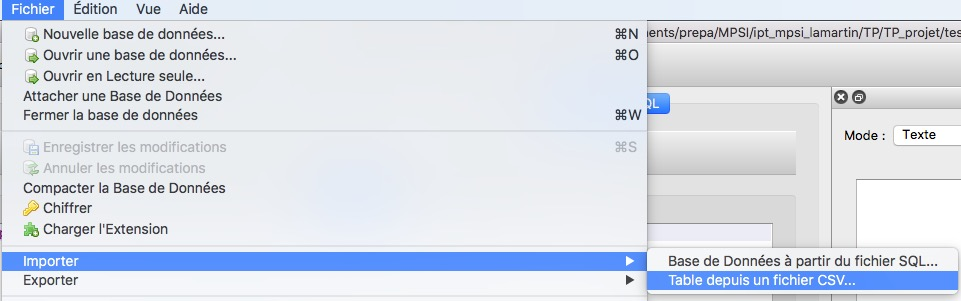
\includegraphics[width=0.8\textwidth]{sql_bw1.jpg}
\end{center}
\item Sélectionner le fichier .csv en question (dans le filtre de selection bien préciser "Tous les fichiers") puis ouvrir.
\begin{center}
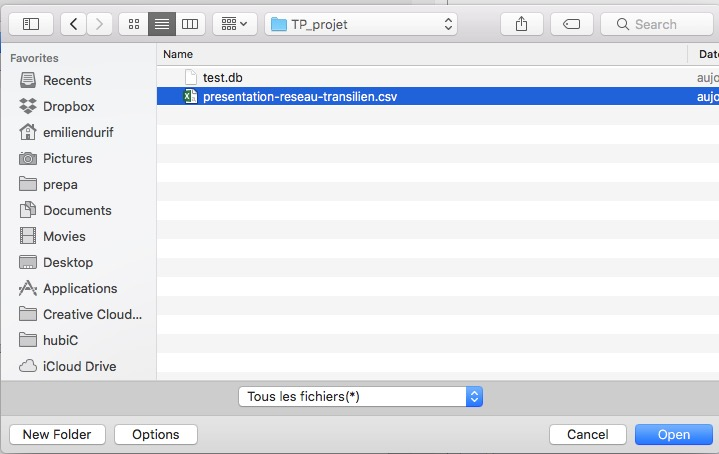
\includegraphics[width=0.5\textwidth]{sql_bw2.jpg}
\end{center}
\item Une fenêtre du paramétrage du fichier .csv apparaît. On peut sélectionner le séparateur de champ ainsi que l'encodage. 
\item Si la première ligne du fichier .csv correspond aux noms des champs, il faut cocher la case "Nom des Col. en 1\up{ère} ligne".
\begin{center}
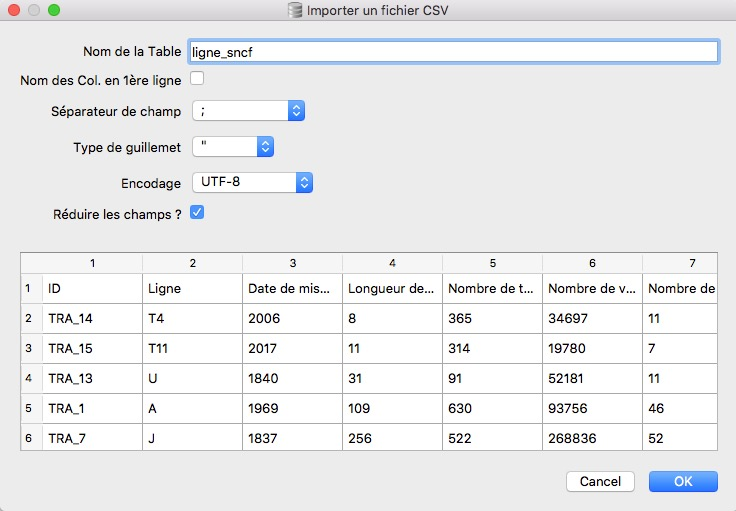
\includegraphics[width=0.5\textwidth]{sql_bw3.jpg}
\end{center}
\item Après validation, la table importée apparaît dans l'onglet "Structure de la Base de Données".
\begin{center}
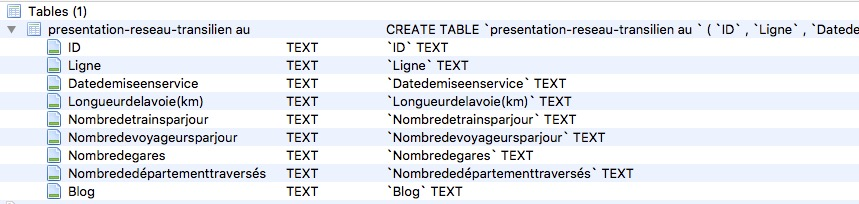
\includegraphics[width=0.8\textwidth]{sql_bw4.jpg}
\end{center}
\end{itemize}